\documentclass{standalone}
\usepackage{tikz}
\usetikzlibrary{intersections}
\usetikzlibrary{calc}
\begin{document}
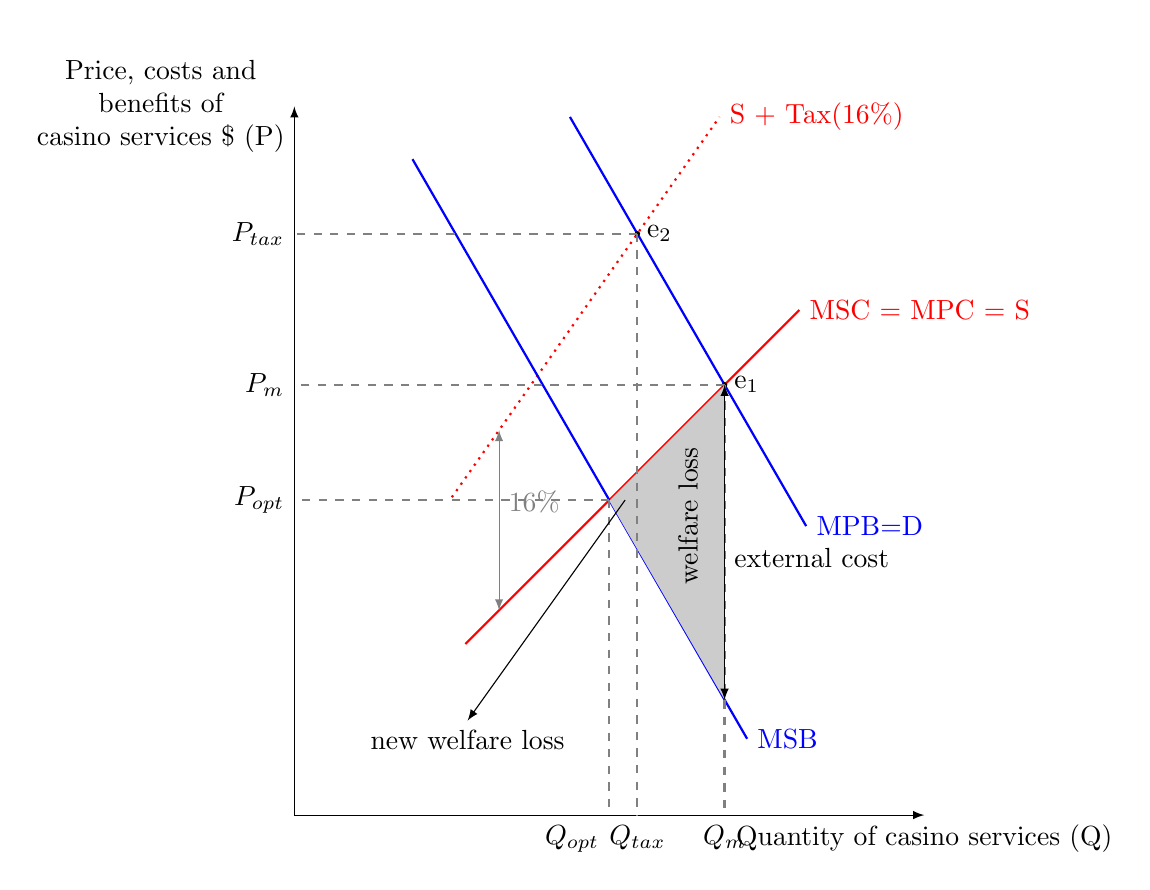
\begin{tikzpicture}[scale=1, >=latex]
    % Axes with padding
    \draw[->] (0,0) -- (8,0) node[below] {Quantity of casino services (Q)};
    \draw[->] (0,0) -- (0,9) node[left, align = center] {Price, costs and\\ benefits of\\ casino services $\mathdollar$ (P)};

    % Original supply point (hidden anchor)
    \coordinate (origin) at (0, 0);

    \path[name path=qopt] (4,0) -- (4,10);
    
    % Supply curves with different slopes through (0.5,2.5)
    \draw[red, thick,name path=s0] ($(5,5)-(45:4)$) -- ($(5,5)+(45:2)$) 
        node[right] {MSC = MPC = S};
    \draw[red, thick, dotted, name path=stax] ($(4,8)-(60:4)-(0,0.5)$) -- ($(4,8)+(60:1)+(0.9,0)$) 
        node[right] {S + Tax(16\%)};
    \draw[blue, thick, name path=mpb]  ($(4,8)+(120:1)$) -- ($(4,8)-(120:5)$)
        node[right] {MPB=D};
    \draw[blue, thick, name path=msb]  ($(4,4)+(120:5)$) -- ($(4,4)-(120:3.5)$)
        node[right] {MSB};
    
    \fill[black, name intersections={of=s0 and mpb, by={e1}}]
        (intersection-1) circle (1pt) node[right] {e\textsubscript{1}};
    \fill[black, name intersections={of=stax and mpb, by={e2}}]
        (intersection-1) circle (1pt) node[right] {e\textsubscript{2}};
    
    \draw[gray, thick, dashed] (e1) -- (e1 -| 0,0)
        node[black, left] {$P_m$};
    \draw[gray, thick, dashed, name path=e1qm] (e1) -- (e1 |- 0,0)
        node[black, below] {$Q_m$};
    
    
    \fill[name intersections={of=e1qm and msb, by={tmp}}];
    \definecolor{lgray}{rgb}{0.8, 0.8, 0.8};
    \fill[lgray] ($(e1) - (0, 0.01)$) -- (tmp) -- (4,3.99) -- cycle;

    %\fill[name intersections={of=stax and msb, by={tmp2}}];
    %\fill[lgray] (e2) -- ($(e1) + (0, 0.01)$) -- (4,4.01) -- (tmp2) -- cycle;

    
    \draw[gray, thick, dashed] (e2) -- (e2 -| 0,0)
        node[black, left] {$P_{tax}$};
    \draw[gray, thick, dashed] (e2) -- (e2 |- 0,0)
        node[black, below] {$Q_{tax}$};
    \draw[gray, thick, dashed] (4,4) -- (0,4)
        node[black, left] {$P_{opt}$};
    \draw[gray, thick, dashed] (4,4) -- (4,0)
        node[black, below left] {$Q_{opt}$};

    \draw[<->] (e1) -- (tmp) node[pos=0.55, right] {external cost};
    \node[rotate=90] at (5,3.8) {welfare loss};
    \draw[->] (4.2, 4.0) -- (2.2, 1.2) node[below] {new welfare loss};
    
    \path[name path=tv] (2.6,0) -- (2.6,10);
    \fill[name intersections={of=tv and stax, by={ar1}}];
    \fill[name intersections={of=tv and s0, by={ar2}}];
    \draw[<->, gray] (ar1) -- (ar2) node[pos=0.4, right]{16\%};

\end{tikzpicture}
\end{document}